
	\section{Estado del arte}\label{sec:stateoftheart}
	
	En esta sección se presentan diversas aplicaciones que tienen como objetivo el facilitar la comunicación entre personas que ocupan el lenguaje de señas con las que no, además, se muestran las técnicas y herramientas usadas para el reconocimiento de voz, así como los algoritmos y diferentes resultados obtenidos.
	
	\subsection{De la aplicación}

	En el mundo hay esfuerzos similares para solucionar los problemas de comunicación de las personas sordas para la integración en la sociedad, los cuales emplean diferentes técnicas y dispositivos para lograr esta interacción.

	\subsubsection*{Institucional}

	\subsubsection*{Traductor de lenguaje sordomudo mediante un guante con sensores y una aplicación móvil}

	En \cite{LunaGarcia2015} se presenta un guante que traduce el lenguaje de señas para sordomudos a personas que no lo conocen, este guante detecta los ademanes realizados por el usuario y los asocia a las letras del alfabeto, formando frases que son transmitidas por Bluetooth a un dispositivo móvil en Android que con ayuda de una aplicación móvil muestra y lee el texto recibido del guante. Básicamente este sistema cuenta con 3 grandes módulos: módulo de sensado, módulo de procesamiento y módulo móvil. Para el sensado de utilizó un total de 11 sensores flex, los cuales presentan una resistencia de acuerdo al ángulo de flexión y se puede decir que su comportamiento es lineal.

	En general, el trabajo pudo realizar la identificación de todas las letras del abecedario menos 4 como por ejemplo la R debido a que tiene una forma complicada de representación que no se pudo caracterizar con el guante, por lo que se dice que el proyecto tuvo una eficiencia del 90 \% (Figura \ref{guanteUPIITA}).

		\begin{figure}[H]
			\centering
			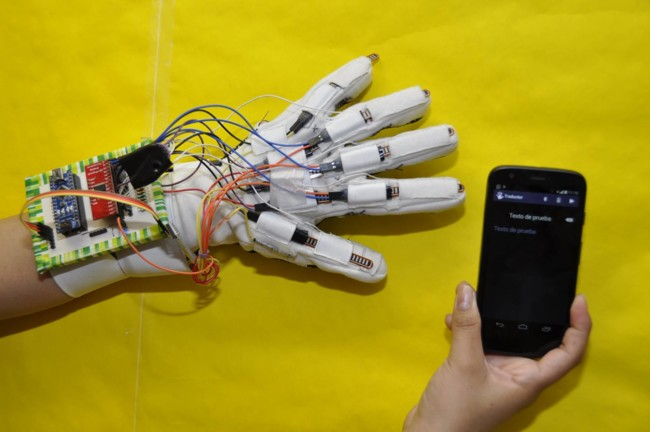
\includegraphics[scale = 0.5]{figures/guanteUPIITA}
			\caption{Traductor de lenguaje sordomudo mediante un guante con sensores y una aplicación móvil.}
			\label{guanteUPIITA}
		\end{figure}	

	\subsubsection*{Traductor del lenguaje de señas mexicano a texto usando FPGAS}

	En la escuela superior de cómputo del Instituto Politécnico Nacional se desarrolló como proyecto de titulación en el año 2003 un dispositivo que reconoce las características del lenguaje de señas mexicano y en tiempo real lo traduce como mensaje de texto. Lo hace mediante una cámara, el dispositivo permite tomar imágenes de las señas de la persona con problemas de audición, se reconocen y procesan en la FPGA para después traducir en forma de texto en tiempo real. El proyecto estuvo a cargo del Dr. Miguel Santiago Suárez Castañón. El prototipo está conformado por una cámara que capta las distintas señas, las traduce y en una pantalla las interpreta como un mensaje. Esto se realizó por medio de algoritmos de reconocimiento de patrones programados para interpretar las imágenes \cite{Yucatan2013} (Figura \ref{traductorESCOM})

		\begin{figure}[H]
			\centering
			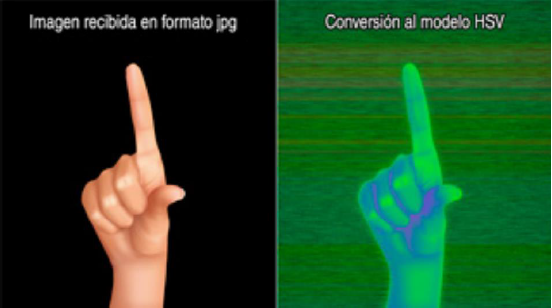
\includegraphics[scale = 0.5]{figures/traductorESCOM}
			\caption{Traductor del lenguaje de señas mexicano a texto usando FPGAS.}
			\label{traductorESCOM}
		\end{figure}

	\subsubsection*{Nacional}

	\subsubsection*{Intérprete de lenguaje de señas}

	Investigadores del Centro de Investigación y tecnología Aplicada (CITA) del Tecnológico de Monterrey, Campus Chihuahua apoyados por CONACYT, desarrollaron una tecnología que aplica la plataforma de videojuegos Kinect de Microsoft para traducir y dar voz a frases con el lenguaje de señas en español.

	Su objetivo es promover la integración social de las personas con discapacidad auditiva, así como mejorar la calidad de vida de los grupos desprotegidos mediante el uso de la tecnología.

	Principalmente el proyecto se basa en el procesamiento de imágenes para el reconocimiento de patrones. De esta forma cuando una persona esté frente al intérprete de lenguaje de señas y realice un movimiento con su cuerpo, el sistema reconoce y procesa los movimientos para posteriormente a través de un sistema de audio escuchar la traducción de los signos o señas.

	Se hace uso de la tecnología de Microsoft kinect Research Software Development Kit (SDK), además del software Language Integrated Query (LINQ), también de Microsoft, tecnología que les permitió implementar modelos conocidos del reconocimiento de imágenes con mayor sencillez \cite{Bustos2012} (Figura \ref{interpreteMICROSOFT}).

		\begin{figure}[H]
			\centering
			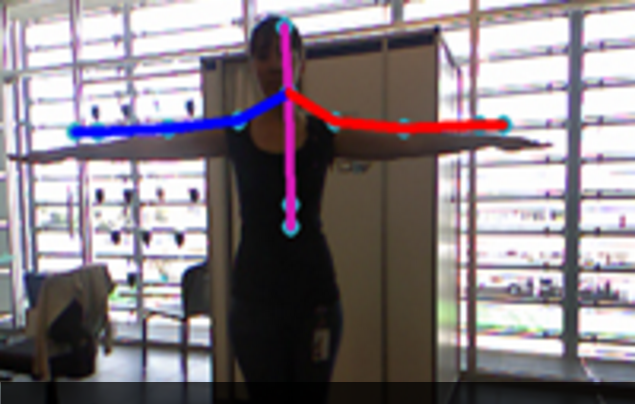
\includegraphics[scale = 0.5]{figures/lenguajeMicrosoft}
			\caption{Intérprete de lenguaje de señas.}
			\label{interpreteMICROSOFT}
		\end{figure}

	\subsubsection*{Internacional}

	\subsubsection*{Software convierte voz en lenguaje de señas para sordos}

	Investigadores de la Facultad de Ingeniería de la Universidad Nacional Autónoma de Honduras (UNAH) desarrollaron una plataforma en computadora capaz de convertir la voz en texto y éste en el lenguaje de señas hondureño para sordos (LESHO). Utiliza un avatar tridimensional que funciona como intérprete virtual, convirtiendo a LESHO el texto generado a partir de la voz del hablante.
	Su objetivo es hacer correr el software en cualquier navegador web y así evitar instalarlo en la computadora. El prototipo se mostró eficaz captando frases cortas en pruebas realizadas en junio del 2014 en los navegadores Chrome y Firefox.
	Se plantea probar el programa en las aulas de la UNAH antes de ampliar el uso, aunque aún falta la traducción de oraciones complejas ya que se requiere el análisis de la oración en español y su traducción al lenguaje de señas. Hasta el momento se han creado y suministrado al programa alrededor de 300 señas \cite{Oliveira2014}.

%	\subsubsection*{Sistema de traducción automática de voz o texto a LSE (Lengua de Signos Española)}
	
%	\subsubsection*{Hand Talk}
	
	\subsection{Del reconocimiento de voz}\label{sub:sr}

	En cuanto al ASR se han realizado diversos trabajos empleando diferentes técnicas de reconocimiento, así como también de extracción de características. En esta sección se muestran algunos trabajos enfocados al SR.

	\subsubsection*{Speech Recognition System Based on Short-term Cepstral Parameters, Feature Reduction Method and Artificial Neural Networks \cite{Nawel2016}}\label{sub:sota:Nawel2016}
	
	En este trabajo se desarrolla un ASR basado en parámetros cepstrales de términos cortos esto para identificar deficiencias de la voz como herramienta complementaria para otras técnicas médicas.
	Para esto utiliza y compara los resultados obtenidos al usar los coeficientes MFCC, su primera y segunda derivada, además para detectar las deficiencias se investiga el uso de LDA para mejorar la habilidad de discriminar del sistema. Además de evaluar el sistema en términos de exactitud, sensitividad, especificidad, precisión y área bajo la curva.
	
	Las características de los métodos y técnicas usadas son las siguientes:
	
	\begin{itemize}
	\item	Se ocupó la base de datos \textit{Saarbrucken Voice Database}, que es una colección de señales de voz con transtornos alemanes que contiene 2225 muestras de voz con una tasa de muestreo de 50 kHz y una resolución de 16 bits.
	\item	La extracción de características se hace por medio de MFCC y se calculan 13 coeficientes, su primera derivada y su segunda derivada. Para la optimización de características se emplea el análisis LDA.
	\item	La arquitectura de la red neuronal propuesta es de tres capas, la capa oculta contiene 250 neuronas a la cual se le aplica la función de activación \textit{sigmoid} y la capa de salida que contiene una neurona con función lineal.
	\item	El aprendizaje de la red neuronal es realizado basado en los algoritmos de regularización bayesiana.
	\item	El conjunto de datos se dividió, un 70\% para el entrenamiento y 30\% para la validación.
	\item	Las simulaciones fueron hechas en Matlab 2013a con Intel Core-i7, 2.20 GHzCPU y 4 GB de RAM.
	\end{itemize}
	
	Los resultados obtenidos muestran que el uso de características MFCC, deltas 1 y 2 y LDA tiene mejor resultado (87.82\% de exactitud) contra los 75.13\% haciéndo uso únicamente de MFCC. 
	
	%\subsubsection*{Phoneme Recognition Using Time-Delay Neural Networks \cite{ALEXANDER1989}}
	
	
	
	%\subsubsection*{Global Optimization of a Neural Network-Hidden Markov Model Hybrid \cite{Yosgua1992}}

	\subsubsection*{DEVELOPMENT OF ISOLATED SPEECH RECOGNITION SYSTEM FOR BANGLA WORDS \cite{A30}}\label{sub:sota:A30}
	
		En este trabajo se desarrolla un sistema de reconocimiento de palabras aisladas del idioma bengalí, para este sistema se destacan las siguientes características:
	
	\begin{itemize}
	\item	De 1 a 6 interlocutores.
	\item	Basado en palabras aisladas y en unidades de palabras (subwords).
	\item	El formato de archivo manejado es WAV.
	\item	Las palabras son agrupadas en 3 grupos diferentes de acuerdo al número de sílabas.
	\item	Para la extracción de características se usa MFCC.
	\item	El sistema de reconocimiento usado es la distancia euclidiana.
	\item	En total se tienen 600 palabras distintas.
	\item	Software utilizado es Turbo C
	\end{itemize}
	
	Las condiciones de las palabras grabadas son las siguientes:
	
	\begin{itemize}
	\item	Las muestras de voz fueron grabadas en un laboratorio insonorizado.
	\item	Se usaron micrófonos de proximidad.
	\item	Tarjetas de audio y software de grabación de alta calidad.
	\item	Las palabras se grabaron a una tasa de muestreo de 8 kHz y se codificaron con PCM de 8 bits.
	\end{itemize}
	
	Algunas características del procesamiento son:
	
	\begin{itemize}
	\item	Segmentación de 16 a 32 ms.
	\item	Para el preénfasis se utilizó la siguiente ecuación
		\begin{equation}\label{eq:xxx}
			y(n)=s(n)-C\cdot s(n-1)
		\end{equation}
		Con valores de $C=0.9 - 1.0$
	\item	Se aplicó la ventana Hamming
	\item	Método de reconocimiento aplicado fue la distancia euclidiana.
	\end{itemize}
	
	Las tasas de reconocimiento obtenidas van de 79.11\% para 6 interlocutores con 3600 palabras en la base de datos a 96\% para un interlocutor y 600 palabras en la base de datos.
	
	\subsubsection*{Continuous Bangla Speech Segmentation using Short-term Speech Features Extraction Approaches \cite{A31}}\label{sub:sota:A31}
	
	Para este trabajo presenta la segmentación de palabras del idioma Bangla usando enfoques de extracción de características.
	
	Las características del dominio del tiempo usadas son la energía y la tasa de cruces por cero de una señal de tiempo corto, por otro lado, en el dominio de la frecuencia se hace uso del centroide espectral y el flujo espectral.
	
	Algunas características de este trabajo son:
	
	\begin{itemize}
	\item	Se utiliza el criterio de umbral dinámico para detectar los bordes de la palabra.
	\item	El interlocutor es un hombre y las muestras se graban a una frecuencia de muestreo de 16 kHz y el tamaño de la muestra es de 8 bits.
	\item	Tamaño del segmento de 50 ms y un traslape de 10 ms, además de usar una ventana rectangular.
	\item	El proceso se lleva a cabo en Matlab 7.12.0.
	\item	El proceso es el siguiente: Adquisición del habla, pre-procesamiento de la señal, extracción de características, cálculo del histograma, umbral dinámico y post-procesamiento.
	\end{itemize}
	
	La tasa de segmentación presentada es de 96.25\%.
	
	\subsubsection*{An Efficient Noise-Robust Automatic Speech Recognition System using Artificial Neural Networks \cite{A3}}\label{sub:sota:A3}
	
	En este trabajo se presenta una técnica de reconocimiento para señales con ruido, se trabaja con 65 palabras diferentes y con una relación señal a ruido de hasta -5dB, se utilizaron los coeficientes MFCC como características para el reconocimiento de voz, la red neuronal empleada es Backpropagation y diversos algoritmos de entrenamiento fueron empleados, los cuales son:
	
	\begin{itemize}
	\item	Polak-Ribiére Conjugate Gradient (CGP).
	\item	Resilient Backpropagation (RP).
	\item	Conjugate Gradient with Powell/Beale Restarts (CGB).
	\item	Scaled Conjugate Gradient backpropagation (SCG).
	\end{itemize}
	
	Las señales de voz utilizadas fueron sintetizadas para obtenerlas lo más limpias posible con un modelo basado en HMM, con una tasa de muestreo de 48000 muestras por segundo con un modelo femenino. Cada palabra se sintetizó 20 veces variando el tono, duración, sonidos sordos y sonoros obteniendo un total de 1300 muestras diferentes. Estas muestras se contaminan con ruido gaussiano reduciendo la SNR de 5dB a -3 dB siendo estas señales las entradas al sistema.
	
	Por otro lado se hace la extracción y compresión de características usando los coeficientes MFCC y para cada vector se calculo su media y varianza, el autor menciona que no utiliza la compresión \textit{K-means} debido a su complejidad y consumo de tiempo.
	
	La estructura de la red neuronal está dada por la entrada la cual toma el vector de características compreso, una capa oculta con función de activación \textit{sigmoid} y la capa de salida con la función de activación \textit{softmax}.
	
	Los resultados presentan que para una longitud de vector de entrada de 20, SNR de -5dB y 30 palabras diferentes con la versión de la red neuronal \textit{Pattern Recognition Network} da un resultado de 94.5\% de exactitud de reconocimiento, para una longitud de 40 del vector de características el mejor resultado es de 98.7\% de exactitud con el algoritmo de entrenamiento SCG.
	
	Finalmente se selecciona la versión de red \textit{Pattern Recognition} y algoritmo de entrenamiento SCG y se hacen pruebas con diferente número de neuronas de la capa oculta y el mejor resultado para un SNR de -3dB y longitud de vector de 40 con 99.6\% son 40 neuronas y para un SNR de -5dB se tuvo el mejor resultado de 99.4\% con 20 neuronas.
	
	\subsubsection*{Combination of Vector Quantization and Hidden Markov Models for Arabic Speech Recognition \cite{A6}}\label{sub:sota:A6}
	
	En este trabajo se presenta el reconocimiento de voz para el árabe usando cuantización vectorial y HMM.
	
	Algunas características de este trabajo son:
	
	\begin{itemize}
	\item	Tasa de muestreo de 11025 Hz
	\item	La etapa de preénfasis se aplicó de acuerdo a la siguiente ecuación
		\begin{equation}\label{eq:xxx}
			\hat{s}(n)=s(n)-a\cdot s(n-1)
		\end{equation}
		Con valor de $a=0.8$
	\item	Los segmentos son de 45 ms espaciadas por 15 ms y un traslape de 30 ms.
	\item	Se aplica la ventana de Hamming
	\item	Para las características se hace un análisis LPC/Cepstral
	\item	Se utilizan los coeficientes Delta Cepstrum
	\item	Se aplica cuantización vectorial
	\item	Las palabras corresponden a los 10 dígitos con 30 interlocutores de entrenamiento y cada uno hace 3 repeticiones por palabra.
	\end{itemize}
	
	En los resultados se muestran dos grupos, los interlocutores que participan en el entrenamiento y los que no. En el primero grupo son los 30 interlocutores y se tiene una tasa de reconocimiento de 95\% y en el segundo grupo se tienen 10 interlocutores con una tasa de reconocimiento de 91\%.
	
	\subsubsection*{COMBINING FUZZY VECTOR QUANTIZATION AND NEURAL NETWORK CLASSIFICATION FOR ROBUST ISOLATED WORD SPEECH RECOGNITION \cite{A7}}\label{sub:sota:A7}
	
	En este trabajo se presenta la combinación de FVQ y NN para llevar a cabo el reconocimiento de voz de palabras aisladas, para esto se emplea una red neuronal multicapa perceptron (MLP) y se compara con FVQ/HMM, agregando ruido blanco o \textit{car noise}.
	
	Las características de la señal de voz son:
	
	\begin{itemize}
	\item	Entrada con banda limitada a 3.6 kHz.
	\item	Tasa de muestreo a 8 kHz con un tamaño de muestra de 16 bits.
	\item	Los segmentos tienen una longitud de 20 ms y un traslape de 10 ms, y cada segmento se analiza con LPC produciendo un vector de 16 LSP y cada conjunto de coeficientes LSP se cuantiza vectorialmente.
	\item	En total se tienen 1040 palabras con 8 interlocutores ingleses, 5 hombres y 3 mujeres, cada interlocutor dio 13 repeticiones de los diez dígitos de las cuales 10 fueron usadas para entrenamiento y 3 para evaluar el desempeño.
	\end{itemize}
	
	Los resultados obtenidos con una SNR de 20dB a 35dB son del 41\% a 95.42\% (el mayor usando FVQ/MLP con 20 nodos ocultos), por otro lado el uso de FVQ/HMM a 35dB de SNR dio como mejor resultado 92.67\% de exactitud de reconocimiento. Estas pruebas se realizaron con ruido blanco.
	
	Para el uso de \textit{car noise} el mejor resultado fue a 35dB de SNR, con el uso de FVQ/HMM se obtuvo una exactitud de 95.83\% y 98.33\% usando FVQ/MLP con  10 nodos ocultos.
	
	\subsubsection*{Combining Neural Network Classification with Fuzzy Vector Quantization and Hidden Markov Models for Robust Isolated Word Speech Recognition \cite{A8}}\label{sub:sota:A8}
	
	En este trabajo se presenta un esquema FVQ/HMM/MLP. Dos conjuntos de entradas fueron usadas en ese experimento, el primer conjunto compuesto de los diez dígitos en inglés, mientras que el segundo conjunto empleó las 26 letras del inglés.
	
	Los resultados obtenidos muestran que se tiene un mejor desempeño de reconocimiento bajo condiciones de ruido que los esquemas FVQ/HMM y FVQ/MLP, el sistema obtuvo una tasa de reconocimiento del 98.33\% a 30 dB de SNR y 90\% a 20dB de SNR cuando se opera en el primer conjunto de palabras.
	
	\subsubsection*{English speech recognition method based on Hidden Markov model \cite{A13}}\label{sub:sota:A13}
	
	En este trabajo se presenta el uso de HMM para reconocimiento de voz en inglés, haciendo pruebas en diferentes ambientes de ruido, además de presentar una mejora a la técnica de HMM.
	
	Para esto se utiliza la base de datos \textit{Aurora 2 English database} la cual se basa en la base de datos \textit{TIDIGITS} submuestreada a 8 kHz y agrega diferentes señales de ruido. La base de datos \textit{TIDIGITS} tiene 326 interlocutores (111 hombres, 114 mujeres, 50 niños y 51 niñas), cada uno pronuncia 77 secuencias de dígitos, para las grabaciones se usó un micrófono \textit{Electro-Voice RE-16 Dynamic Cardiod}, muestreado a 20 kHz.
	
	La mejora al método de HMM es la adición de una capa oculta para representar la evolución del estado de transición.
	
	Los resultados obtenidos con la técnica HMM y HMM mejorada se muestran en la Tabla \ref{tb:hmm}:
	
	% Please add the following required packages to your document preamble:
	% \usepackage{multirow}
	\begin{table}[H]
	\centering
	\caption{Promedio de precisión de reconocimiento}
	\label{tb:hmm}
	\begin{tabular}{|l|l|l|}
	\hline
	\multicolumn{1}{|c|}{\multirow{2}{*}{Ambiente}} & \multicolumn{2}{l|}{Precisión de reconocimiento} \\ \cline{2-3} 
	\multicolumn{1}{|c|}{}                          & HMM                  & HMM mejorado              \\ \hline
	Subway                                          & 44.87\%              & 49.98\%                   \\ \hline
	Babble                                          & 45.72\%              & 49.25\%                   \\ \hline
	Car                                             & 52.79\%              & 57.95\%                   \\ \hline
	Exhibition hall                                 & 55.27\%              & 59.84\%                   \\ \hline
	\end{tabular}
	\end{table}


	A continuación se presenta la tabal comparativa de los artículos presentados.
	
	\newpage
	 \begin{landscape}
	\begin{table}[]
\centering
\caption{Tabla comparativa de técnicas de reconocimiento de voz}
\label{tb:comparativaSOA}
\scalebox{0.9}{
\begin{tabular}{|l|l|l|l|l|}
\hline
Trabajo  & Pre-procesamiento                                                                                                                                                        & \begin{tabular}[c]{@{}l@{}}Técnica de\\ reconocimiento\end{tabular}                                                               & Características                                                                                                                                                                                                      & Resultados                                                                                                       \\ \hline
{[}11{]} & \begin{tabular}[c]{@{}l@{}}MFCC (13 coeficientes)\\ primera y segunda derivada\end{tabular}                                                                              & \begin{tabular}[c]{@{}l@{}}Red neuronal,\\ \\ aprendizaje basado en\\ algoritmos de regularización\\ bayesiana\end{tabular}       & \begin{tabular}[c]{@{}l@{}}Base de datos \\ \textit\{Saarbrucken Voice Database\}\\ Tasa de muestreo a 50 kHz\\ y resolución de 16 bits\end{tabular}                                                                 & \begin{tabular}[c]{@{}l@{}}Uso de MFCC, deltas 1 y 2\\ y análisis LDA, exactitud\\ de 87.82\%\end{tabular}       \\ \hline
{[}12{]} & \begin{tabular}[c]{@{}l@{}}Extracción de características\\ MFCC\\ Ventana Hamming\\ Segmentación de 16 a 32 ms\end{tabular}                                              & Distancia euclidiana                                                                                                              & \begin{tabular}[c]{@{}l@{}}1 a 6 interlocutores\\ Tarjetas de audio y software de \\ alta calidad\\ 600 palabras distintas\\ Tasa de muestreo a 8 kHz\\ y resolución de 8 bits\end{tabular}                          & \begin{tabular}[c]{@{}l@{}}Resultados de 96\% con\\ 1 interlocutor y 79.11\% con\\ 6 interlocutires\end{tabular} \\ \hline
{[}13{]} & \begin{tabular}[c]{@{}l@{}}Segmentación de palabras.\\ Segmentos de 50 ms y \\ traslape de 10 ms\end{tabular}                                                            & \begin{tabular}[c]{@{}l@{}}Segmentación con umbral\\ dinámico\end{tabular}                                                        & \begin{tabular}[c]{@{}l@{}}Uso de 4 características\\ energía\\ tasa de cruces por cero\\ flujo espectral\\ y centroide espectral\end{tabular}                                                                       & Resultados de 96.25\%                                                                                            \\ \hline
{[}14{]} & \begin{tabular}[c]{@{}l@{}}Extracción de características\\ MFCC, compresión con\\ media y varianza\end{tabular}                                                          & \begin{tabular}[c]{@{}l@{}}Red neuronal backpropagation\\ con algoritmos de \\ entrenamiento:\\ CGP\\ RP\\ CGB\\ SCG\end{tabular} & \begin{tabular}[c]{@{}l@{}}Mejores resultados con \\ \textit\{Pattern Recognition Network\}\\ 65 palabras diferentes\\ con 20 repeticiones cada una,\\ variando tono, duración, etc.\\ SNR de -5 a 5 dB\end{tabular} & \begin{tabular}[c]{@{}l@{}}Para SNR de -5dB se tiene\\ resultado de 99.4\%\end{tabular}                          \\ \hline
{[}15{]} & \begin{tabular}[c]{@{}l@{}}Análisis LPC y delta cepstrum\\ Ventana de Hamming\\ Tasa de muestreo de 11025 kHz\\ Segmentos de 45 ms con \\ traslape de 30 ms\end{tabular} & \begin{tabular}[c]{@{}l@{}}HMM con cuantización \\ vectorial\end{tabular}                                                         & \begin{tabular}[c]{@{}l@{}}30 interlocutores y palabras\\ correspondientes a los 10 dígitos\\ cada uno hace 3 repeticiones de cada\\ palabra\end{tabular}                                                            & \begin{tabular}[c]{@{}l@{}}Tasa de reconocimiento de \\ 91\% a 95\%\end{tabular}                                 \\ \hline
{[}16{]} & \begin{tabular}[c]{@{}l@{}}Análisis LPC a 16 coeficientes\\ Segmentos de 20 ms y \\ traslape de 10 ms\end{tabular}                                                       & \begin{tabular}[c]{@{}l@{}}FVQ/MLP\\ FVQ/HMM\end{tabular}                                                                         & \begin{tabular}[c]{@{}l@{}}1040 palabras\\ 8 interlocutores\\ 13 repeticiones de los 10 dígitos\\ SNR de 20dB a 35dB\end{tabular}                                                                                    & \begin{tabular}[c]{@{}l@{}}Mejor resultado con \\ FVQ/MLP de 98.33\% a 35 dB\\ de SNR\end{tabular}               \\ \hline
{[}17{]} & --                                                                                                                                                                       & FVQ/HMM/MLP                                                                                                                       & 10 dígitos en inglés                                                                                                                                                                                                 & \begin{tabular}[c]{@{}l@{}}Reconocimiento de 98.33\%\\ a 30dB de SNR\end{tabular}                                \\ \hline
{[}18{]} & Muestreo de 8 kHz                                                                                                                                                        & HMM y HMM mejorada                                                                                                                & \begin{tabular}[c]{@{}l@{}}Base de datos \\ \textit\{Aurora 2 English database\}\end{tabular}                                                                                                                        & Tabla                                                                                                            \\ \hline
\end{tabular}}
\end{table}

\end{landscape}
	
%	\subsection{De reconocimiento}
	
%	Diferentes implementaciones de un ASR se han llevado a cabo con diferentes técnicas, algoritmos y herramientas, a continuación se mencionan algunos resultados obtenidos.
	
%	En \cite{A1} se define ASR (Automatic speech recognition) como la transcripción independiente, computarizada del lenguaje hablado en texto legible en tiempo real.
	
%	Aquí se mencionan los diferentes métodos usados para ASR, dentro de los cuales destaca el uso de HMM ya que la voz puede visualizarse como una señal estacionaria pieza por pieza o una señal estacionaria de corto tiempo. También menciona que el uso de redes neuronales puede ser eficiente en SR pero no en tareas de reconocimiento continuo, debido a su falta de capacidad para modelar dependencias temporales.
	
%	Uno de los componentes principales del ASR es la extracción de características ya que este proceso usa la información más relevante de la señal de voz y ayuda a distinguir entre diferentes unidades lingüísticas y elimina ruido externo, perturbaciones y emociones. Las técnicas de extracción más comunes  son MFCC, LPC, LPCC, de las cuales \cite{A1} menciona que la técnica MFCC ha sido comprobada como el estado del arte en cuanto a extracción de características desde que se basa en el sistema de audición humana y trabaja sobre una escala de frecuencias llamada \textit{Mel}. Para lenguajes como el inglés, chino, japonés e incluso el hindi se han tenido eperimentalmente resultados del 80\% de eficiencia contral el 60\% que tienen LPC y LPCC.
	

	
	